\documentclass{article}

\usepackage[margin=1.6cm]{geometry}
\usepackage{amsmath,amssymb}
\usepackage{float}
\usepackage{graphicx}
\usepackage{fancyhdr}
\pagestyle{fancy}
\usepackage{tcolorbox,listings}
\usepackage{color}
\usepackage{hyperref}
\renewcommand\headrulewidth{1pt}
\usepackage{marvosym}
\usepackage{xcolor}
\usepackage{tikz}
%\usepackage{babel}
\usepackage[french]{babel}
\usepackage[babel=true,kerning=true]{microtype}
\usepackage{afterpage}

\newcommand\myemptypage{
    \null
    \thispagestyle{empty}
    \addtocounter{page}{-1}
    \newpage
    }

\usetikzlibrary{
  arrows,
  calc,
  shapes.geometric,
  shapes.misc,
  shapes.symbols,
  shapes.arrows,
  automata,
  through,
  positioning,
  scopes,
  decorations.shapes,
  decorations.text,
  decorations.pathmorphing,
  shadows}

\definecolor{darkWhite}{rgb}{0.94,0.94,0.94}
 
\lstset{
    backgroundcolor=\color{darkWhite},
    breakatwhitespace=false,
    breaklines=true,
    captionpos=b,
    commentstyle=\color{green},
    deletekeywords={...},
    escapeinside={\%*}{*)},
    extendedchars=true,
    keepspaces=true,
    keywordstyle=\color{blue},
    %language=Python,
    morekeywords={*,...},
    showspaces=false,
    showstringspaces=false,
    showtabs=false,
    stepnumber=1,
    stringstyle=\color{gray},
    tabsize=4,
}
 
\lstdefinestyle{frameStyle}{
    basicstyle=\sffamily,
    numbers=left,
    numbersep=20pt,
    numberstyle=\tiny\color{black}
}
 
\tcbuselibrary{listings,skins,breakable}
 
\newtcblisting{customFrame}{
    arc=0mm,
    top=0mm,
    bottom=0mm,
    left=3mm,
    right=0mm,
    width=\textwidth,
    listing only,
    listing options={style=frameStyle},
    breakable
}

\fancyhead[L]{ALLEMAND Fabien\\LEBOT Samuel}
\fancyhead[C]{Compilation}
\fancyhead[R]{
\includegraphics[scale=0.08]{img/logo_UFR_1.png}}
\fancyfoot[L]{Rapport de Projet}
\fancyfoot[R]{\today}

\begin{document}

\newpage
\thispagestyle{empty}
\addtocounter{page}{-1}
\begin{center}
	\baselineskip=50pt
	\vspace*{1cm}
	\textbf{{\Huge Compilation}}\\
	\vspace*{0.25cm}
	\textbf{{\Huge Rapport de Projet}}\\
	\vspace*{0.25cm}
	\begin{minipage}[c]{.46\linewidth}
        \centering
        \textbf{Equipe:}\\
		ALLEMAND Fabien\\
        ??? Samuel
    \end{minipage}
\end{center}
\vspace{0.1cm}

\begin{figure}[H]
\centering
\centerline{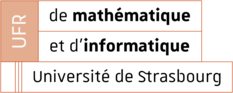
\includegraphics[scale=1.]{img/logo_UFR_2.png}}
\end{figure}

% \newpage
% \myemptypage

\pagenumbering{roman}

% \newpage
% \myemptypage

\newpage
% \addcontentsline{toc}{section}{Table des matières}
\renewcommand{\contentsname}{Table des matières}
\tableofcontents

\newpage
\addcontentsline{toc}{section}{Liste des figures}
\renewcommand{\listfigurename}{Liste des figures}
\listoffigures

\pagenumbering{arabic}

\newpage
\section{Introduction}

\paragraph{}
La compilation consiste à traduire un code source lisible par un humain en un code exécutable par un ordinateur. C'est à dire transformer un fichier texte contenant des instructions écrites dans un langage de programmation en un fichier binaire.

\paragraph{}
Ce projet consiste à écrire un compilateur pour un langage de programmation impératif simple appelé SoS qui utilise une syntaxe et des fonctionnalités issues d'un sous-ensemble de langage shell
unix (Sous-Shell).\\
\'Ecrit en C et en utilisant les outils \textsf{Flex} et \textsf{Bison}, le compilateur est capable de traduire un programme écrit en SoS en une suite d'instructions MIPS pouvant être exécutées à l'aide d'un simulateur.

\paragraph{}
Dépôt Git: \url{https://github.com/FABallemand/ProjetCompilation}

\newpage
\section{Analyse Lexicale}

\paragraph{}
La première étape de la compilation consiste à analyser les unités lexicales contenues dans un programme, c'est à dire découper le programme en blocs de taille la plus petite possible selon la syntaxe du langage de programmation.

\paragraph{}
L'analyse lexicale est réalisée à l'aide de \textsf{Flex}. Cet outil permet de définir des unités lexicales sous formes d'expressions rationnelles et d'associer une action à chacune d'elles.

\paragraph{}
On peut donc définir les unités lexicales utilisées dans un programme écrit en SoS. Dans le fichier \textsf{fsos.lex}, on définit tout d'abord les unités lexicales réservées au langage:
\begin{itemize}
    \item Les symboles (\textbf{+}, \textbf{-}, \textbf{*}, \textbf{()}...)
    \item Les mots clés (\textbf{if}, \textbf{for}, \textbf{test}...)
\end{itemize}
Puis les unités lexicales définies par l'utilisateur:
\begin{itemize}
    \item Chaines de caractères
    \item Nombres
    \item Identifiants de variables ou de fonctions
    \item Commentaires
    \item Espaces et tabulations
\end{itemize}

\paragraph{}
On associe ensuite une action à chaque unité lexicale.\\
Pour les unités lexicales réservées au langages, cela consiste à renvoyer un \textit{TOKEN}, c'est à dire une valeur numérique correspondant à une unité lexicale.
\begin{figure}[H]
\begin{lstlisting}
\+ return PLUS;
if return IF;
\end{lstlisting}
\caption{Exemple d'action \textsf{Flex} pour le symbole \textbf{+} et le mot clé \textbf{if}}
\end{figure}

Les unités lexicales ayant une valeur définie par l'utilisateur doivent être ignorées ou transmises (à l'aide de \textsf{yylval}, \textsf{yytext} ainsi qu'un TOKEN).
\begin{figure}[H]
\begin{lstlisting}
#[^\n]*\n ;
(([1-9][0-9]*)|0) {yylval.val = strdup(yytext); return INTEGER;}
\end{lstlisting}
\caption{Exemple d'action \textsf{Flex} pour les commentaires et les entiers}
\end{figure}

\noindent
\begin{minipage}[!hc]{0.12\textwidth}
   \textbf{Remarque}
\end{minipage}
\vrule\enskip\vrule\quad\begin{minipage}{\dimexpr 0.87\textwidth-0.8pt-1.5em}
Les unités lexicales qui ne sont pas reconnues par l'analyseur lexical sont considérées incorrectes pour un programme SoS et mettent fin à la compilation.
\end{minipage}

\noindent
\begin{minipage}[!hc]{0.12\textwidth}
   \textbf{Remarque}
\end{minipage}
\vrule\enskip\vrule\quad\begin{minipage}{\dimexpr 0.87\textwidth-0.8pt-1.5em}
Le symbole terminal \textbf{mot} mentionné dans la grammaire initiale du langage SoS a été supprimé. Ce symbole était en conflit avec les symboles terminaux \textbf{entier} et \textbf{chaine}.\\
Ainsi la grammaire modifiée utilisée par le compilateur marque les chaines de caractères avec des simple/double quotes ce qui permet de lever toute ambiguité entre les chaines de caractères, les entiers et les identifiants de variables ou de fonctions lors de l'analyse lexicale.\\
Cette distinction ne correspond pas à un type mais plutôt à un marquage pour autoriser certaines opérations pour une variable. (Chaque variable correspondant à une chaine de caractères initialement.)
\end{minipage}

\paragraph{}
Les valeurs renvoyées par l'analyseur lexical \textsf{Flex} sont transmises à l'analyseur syntaxique.

\newpage
\section{Analyse Syntaxique}

\paragraph{}
Après avoir déterminé les blocs de taille minimale composant le programme, il faut vérifier s'ils sont assemblés de façon correcte. C'est à dire si le programmeur a écrit des instructions correctes et agencées convenablement selon la grammaire du langage de programmation.

\paragraph{}
L'analyse syntaxique est réalisée à l'aide de \textsf{Bison}, un outil permettant de définir la grammaire d'un langage de programmation et de définir des actions à effectuer pour chaque règle rencontrée dans le programme.

\paragraph{}
L'exemple de règle ci-dessous correspond à la multiplication de deux entiers. On y trouve:
\begin{itemize}
    \item Une instruction qui permet d'afficher la règle lorsqu'elle est utilisée (utilisé pour du debuggage)
    \item La création d'une opérande de type variable utilisable dans une instruction de code intermédiaire
    \item Un appel à la fonction \textsf{genCode} qui permet de générer le code intermédiaire (code à trois adresses) correspondant.
    \item Des affectations de valeurs de l'élément de droite à l'élément de gauche de la règle selon leur type
\end{itemize}
\begin{figure}[H]
\begin{lstlisting}
produit_entier
: produit_entier STAR operande_entier
{
    if(DEBUG)
        printRule("produit_entier STAR operande_entier");
    $$.firstquad = $1.firstquad;
    struct quadop result = quadop_var(newtemp());
    genCode(quad_new(Q_MUL, $1.result, $3.result, result));
    $$.result = result;
}
\end{lstlisting}
\caption{Exemple d'action \textsf{Bison} pour la multiplication de deux entiers}
\end{figure}

\paragraph{}
La première partie du fichier \textsf{bsos.y} permet de définir des propriétés de la grammaire (priorité des opérations) ainsi que des outils pour l'analyse syntaxique (TOKEN et types d'éléments de règles).\\
Les types définis dans la section \textsf{\%union} permettent d'utiliser chaque élément de règle comme une structure pour y stocker des information à porpager lors de la compilation.
\begin{figure}[H]
\begin{lstlisting}
%union{
    struct {
        size_t firstquad;
        struct quadop result;
    } expr_val;
}

%type <expr_val> produit_entier
\end{lstlisting}
\caption{Déclaration du type \textsf{expr\_val} dans le fichier \textsf{Bison}}
\end{figure}
Dans l'exemple précédent on utilise \textsf{dollar dollar} pour accéder aux champs de \textsf{produit\_entier} et y affecter les valeurs de l'addresse du premier \textit{quadruplet} (code à trois adresses) correspondant à la multiplication et le resultat de cette multiplication.\\

\paragraph{}
La partie la plus importante de fichier \textsf{Bison} (la deuxième) contient toutes les règles de la grammaire et leurs actions.\\
\`A cette étape de la compilation, on génère du code intermédiaire grâce à la fonction \textsf{genCode}. Les différents types de quadruplets (\textsf{Q\_ADD}, \textsf{Q\_EQUAL\_STRING}, \textsf{Q\_GOTO}...) et types d'opérandes de quadruplets (\textsf{QO\_CST}, \textsf{QO\_VAR}, \textsf{QO\_UNKNOWN}...) sont définis dans le fichiers \textsf{quad.h}.\\
L'adresse d'une instruction correspond à sa position dans un tableau de quadruplets contenant toutes les instructions du programme. Certaines instructions, notamment les \textsf{Q\_GOTO}, contiennent des opérandes qui ne sont pas connues au moment où elles sont compilées. Il faut donc les enregistrer dans le quadruplet comme \textsf{QO\_UNKNOWN}, les enregistrer dans le membre gauche de la règle dans un liste d'opérandes à compléter (\textsf{next}, \textsf{ltrue} ou \textsf{lfalse}) et les compléter par la suite grâce à la fonction \textsf{complete}.
\paragraph{}
C'est aussi à cette étape de la compilation que la table des symboles est créée. Cette structure a pour but d'enregistrer les variables déclarées dans le programme SoS à compiler ainsi que leur portées. On utilise pour cela une pile de contextes (voir \textsf{symbol\_table.h} et \textsf{symbol\_table.c}). Dans l'exemple ci-dessous, on constate que la fonction \textsf{pushContext} est utilisée pour empiler le contexte global.
\begin{figure}[H]
\begin{lstlisting}
initialisation 
: %empty
{
    if(DEBUG)
        printRule("empty (initialisation)");
    pushContext();
    newName(S_GLOBAL, status, VAR, 0);
    genCode(quad_new(Q_AFFECT, quadop_cst(zero), quadop_empty(), quadop_var(status)));
}
\end{lstlisting}
\caption{Actions réalisées pour initialiser un programme lors de l'analyse syntaxique}
\end{figure}
On remarque aussi dans l'exemple ci-dessus l'appel à la fonction \textsf{newName} qui permet de créer une nouvelle variable dans la table des symboles, ici pour créer la variable \textsf{?} (identifiant invalide pour un utilisateur)qui contient le status (le code de retour du programme). Une stratégie similaire est utilisée pour le code retour d'une fonction.\\
La fonction \textsf{newName} est aussi utilisée pour créer des variables temporaires dans le table des symboles qui ont elles aussi un identifiant invalide pour un utilisateur afin d'éviter tout conflit entre varibles.\\
Par la suite, on peut vérifier si une variable est dans le contexte voulu grâce à la fonction \textsf{lookUp} et en précisant le niveau de contexte souhaité (courrant et/ou global).

\newpage
\section{Génération de Code MIPS}

\newpage
\section{Conclusion}

\paragraph{}
Le compilateur que nous avons écrit (bien qu'assez peu performant) permet de compiler correctement des programmes écrits dans le langage SoS.\\
L'analyseur lexical et l'analyseur syntaxique permettent de générer du code intermédiaire. Nous avons accordé une attention particulière à la table de symboles et à la gestion des contextes.\\
La traduction en code MIPS est assurée par un programme en C qui traduit le code intermédiaire en MIPS et une bibliotèque de fonctions MIPS.

\paragraph{}
La compilation est encore de nos jours un domaine de recherche en plein essor. De nouvelles contraintes liées à la performance mais aussi à l'efficacité énergétique du code généré donnent lieu à de nouvelles méthodes d'optimisation parfois très complexes.\\
Cet aspect de la compilation n'a malheureusment pas pu être abordée lors de ce projet. Sans doute de nombreuses améliorations peuvent être apportées à ce compilateur!

% \newpage
% \addcontentsline{toc}{section}{Bibliographie}
% \renewcommand{\refname}{Bibliographie}
% \bibliographystyle{plain}
% \bibliography{bibliographie}

% \newpage
% \myemptypage

% \newpage
% \input{src/annexes.tex}

\end{document}